\section{Earthquake Safety}
\label{ild:sec:earthquake}
Japan is one of most seismically active regions in the world. The proposed site for the ILC in the Kitakami mountains of northern Honshu has been especially selected putting emphasis on benign seismic conditions. Earthquake history has been taken into account as well as recent surveys on active tectonic faults. Nevertheless, earthquakes can occur and need to be taken into account. Figure~\ref{ild:fig:integration:earthquake_map} shows all earthquakes that were detected during 30 days in winter 2018/2019 in northern Honshu. The ILD interaction region is in the region around (39N, 141,5E).

\begin{figure}[h!]
\centering
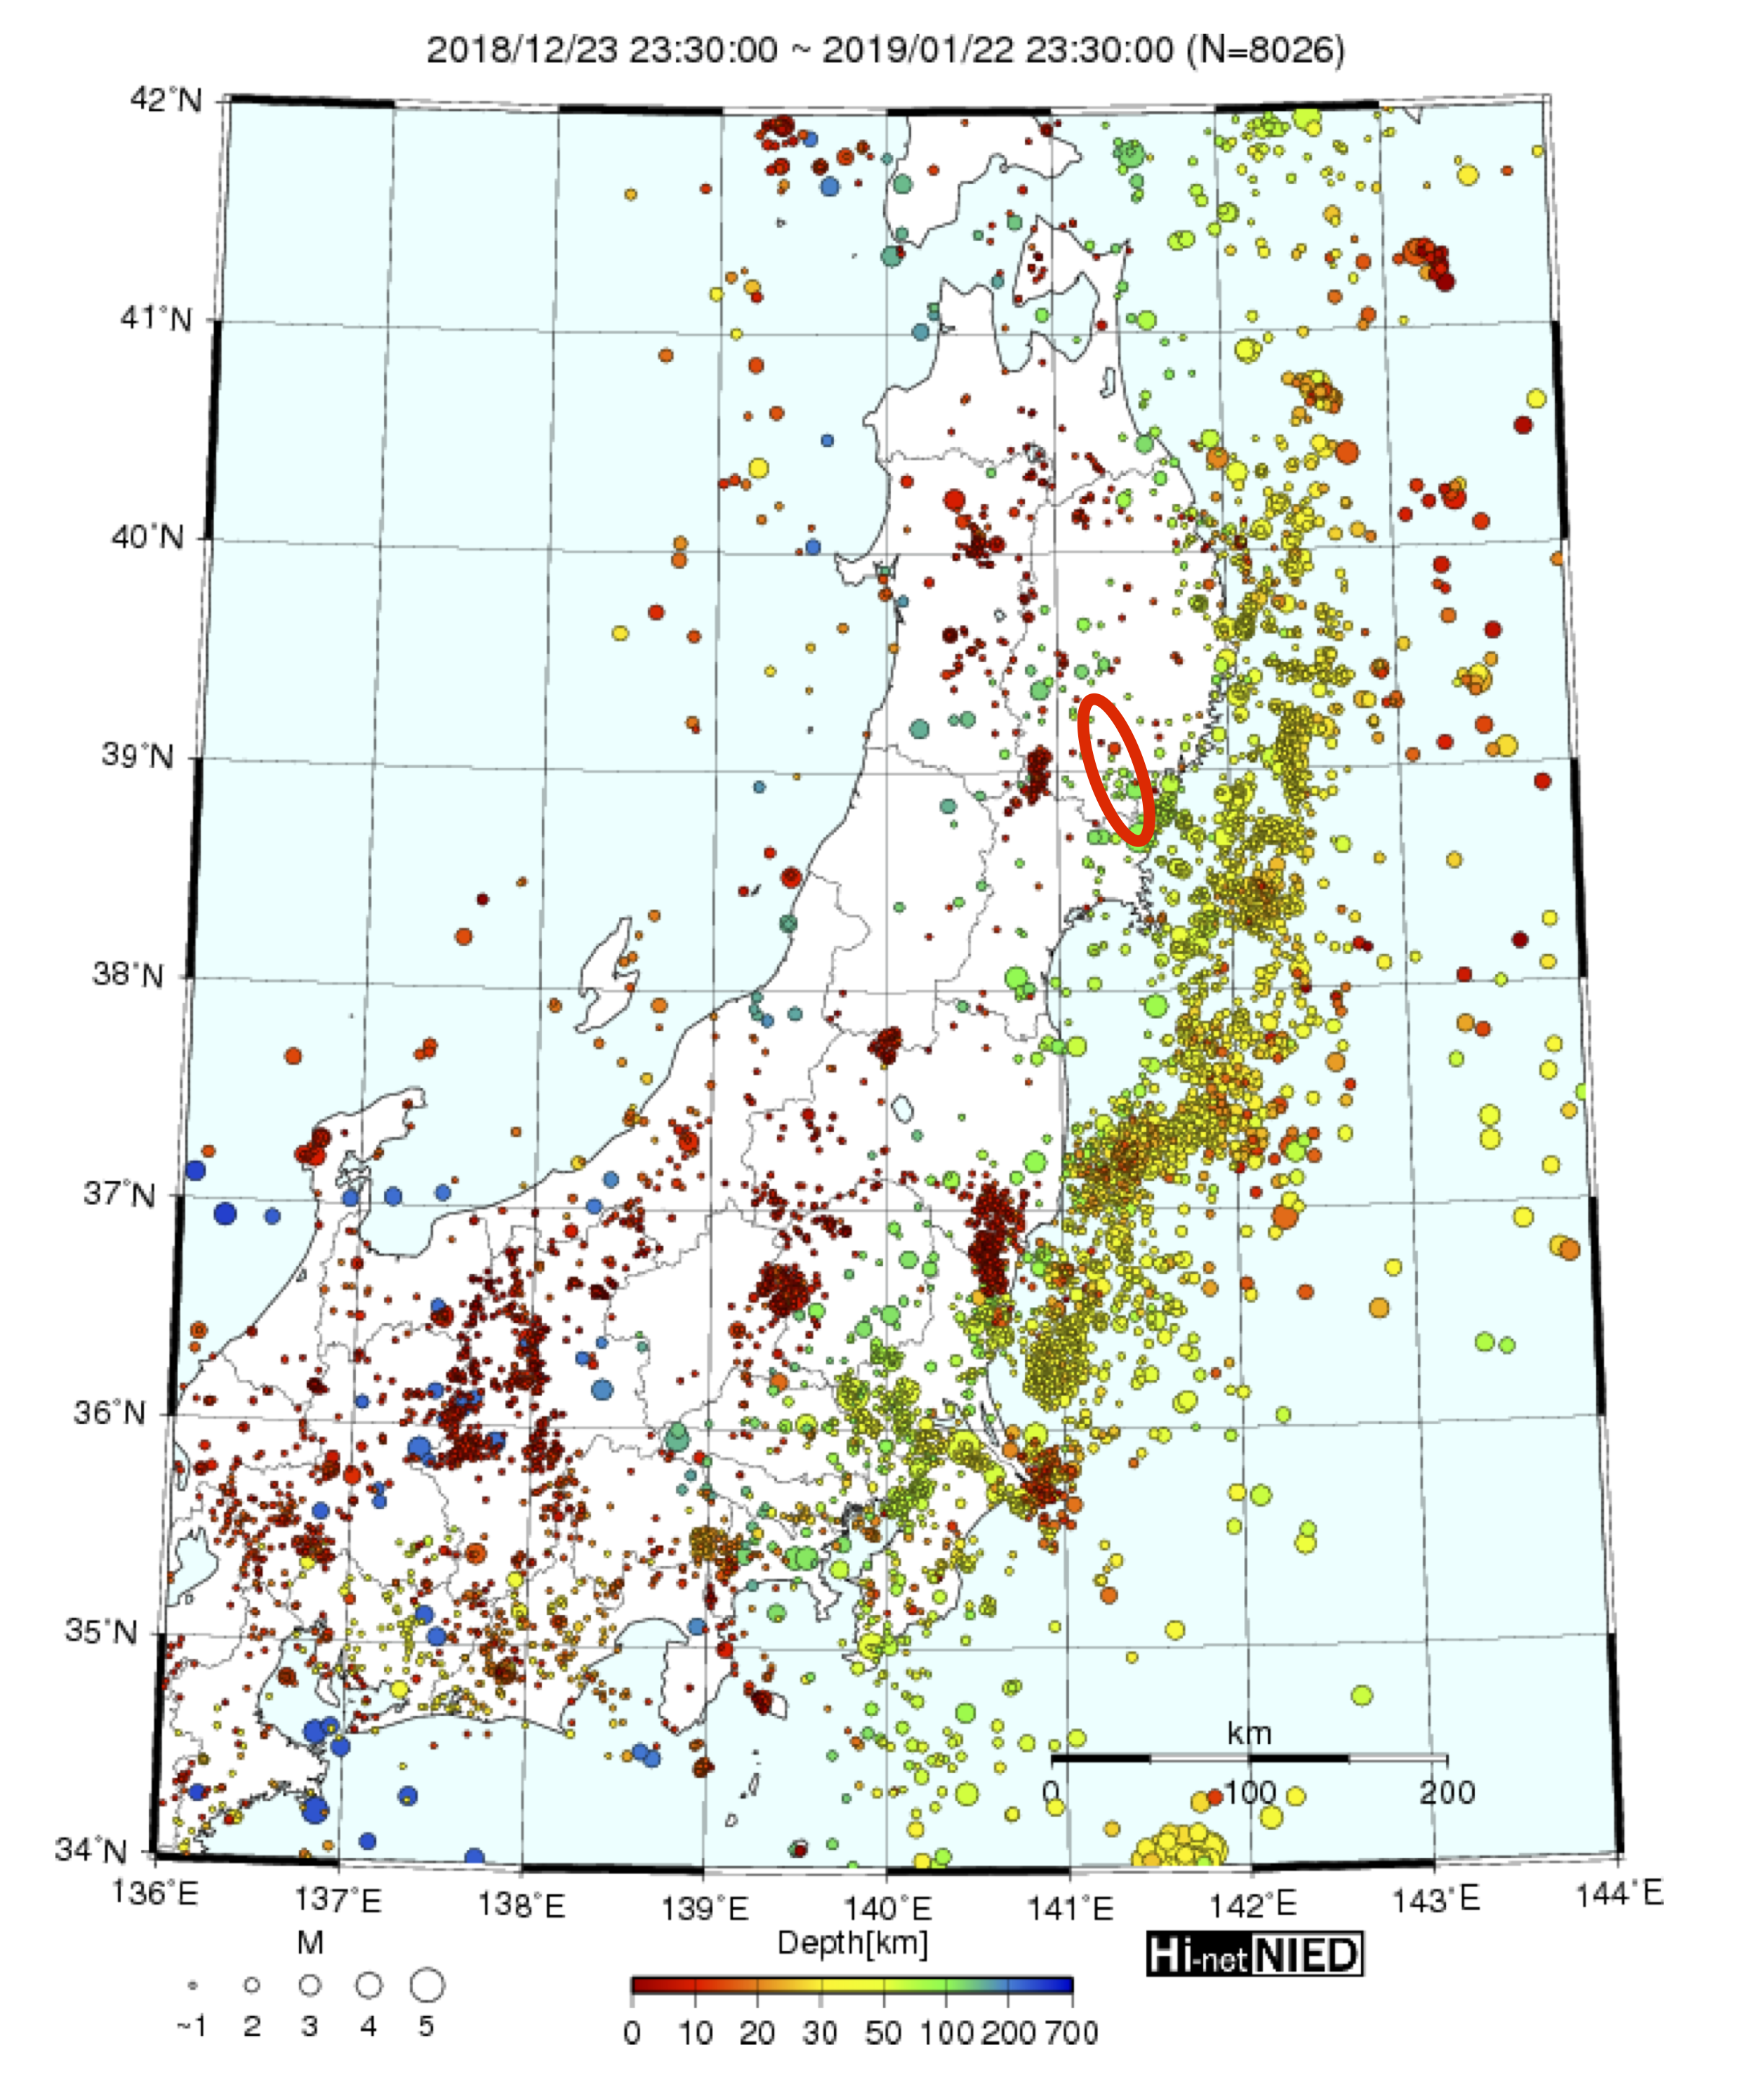
\includegraphics[width=0.8\hsize]{Integration/fig/earthquake_map.png}

\caption{\label{ild:fig:integration:earthquake_map}Map of northern Honshu with all detected earthquakes between 23rd December 2018 and 23rd January 2019 (30 days)~\cite{ild:bib:hi-net}. The ILC site is indicated by the red ellipse.}
\end{figure}

\subsection{Structural Design}

Emphasis has been put on the design of the ILD detector with respect to earthquake safety in view of operability of the detector as well as disaster prevention. General rules are provided by the ISO3010 standard: "Bases for design of structures -- seismic actions on structures". The ISO standard states two basic principles:
\begin{itemize}
\item The structure should not collapse nor experience other similar forms of structural failure due to severe earthquake ground motions that could occur at the site (ultimate limit state: ULS).
\item The structure should withstand moderate earthquake ground motions which may be expected to occur at the site during the service life of the structure with damage within accepted limits (serviceability limit state: SLS).
\end{itemize}

The design seismic forces on mechanical structures can be determined by taking into account normalised design response spectra, weighted with load factors that take into account the respective state, ULS or SLS, local conditions and structural factors. In addition, required degrees of reliability of the structures can be taken into account.

An acceleration response spectrum for the SLS state at the Kitakami site is shown in Figure~ \ref{ild:fig:integration:earthquake_spectra} for structures with different damping behaviours. In the ULS state, the accelerations are assumed to be larger by about a factor of two. These type of standard spectra serve as input for the structural studies described in section~\ref{ild:sec:mechanical_structures}.
\begin{figure}[t!]
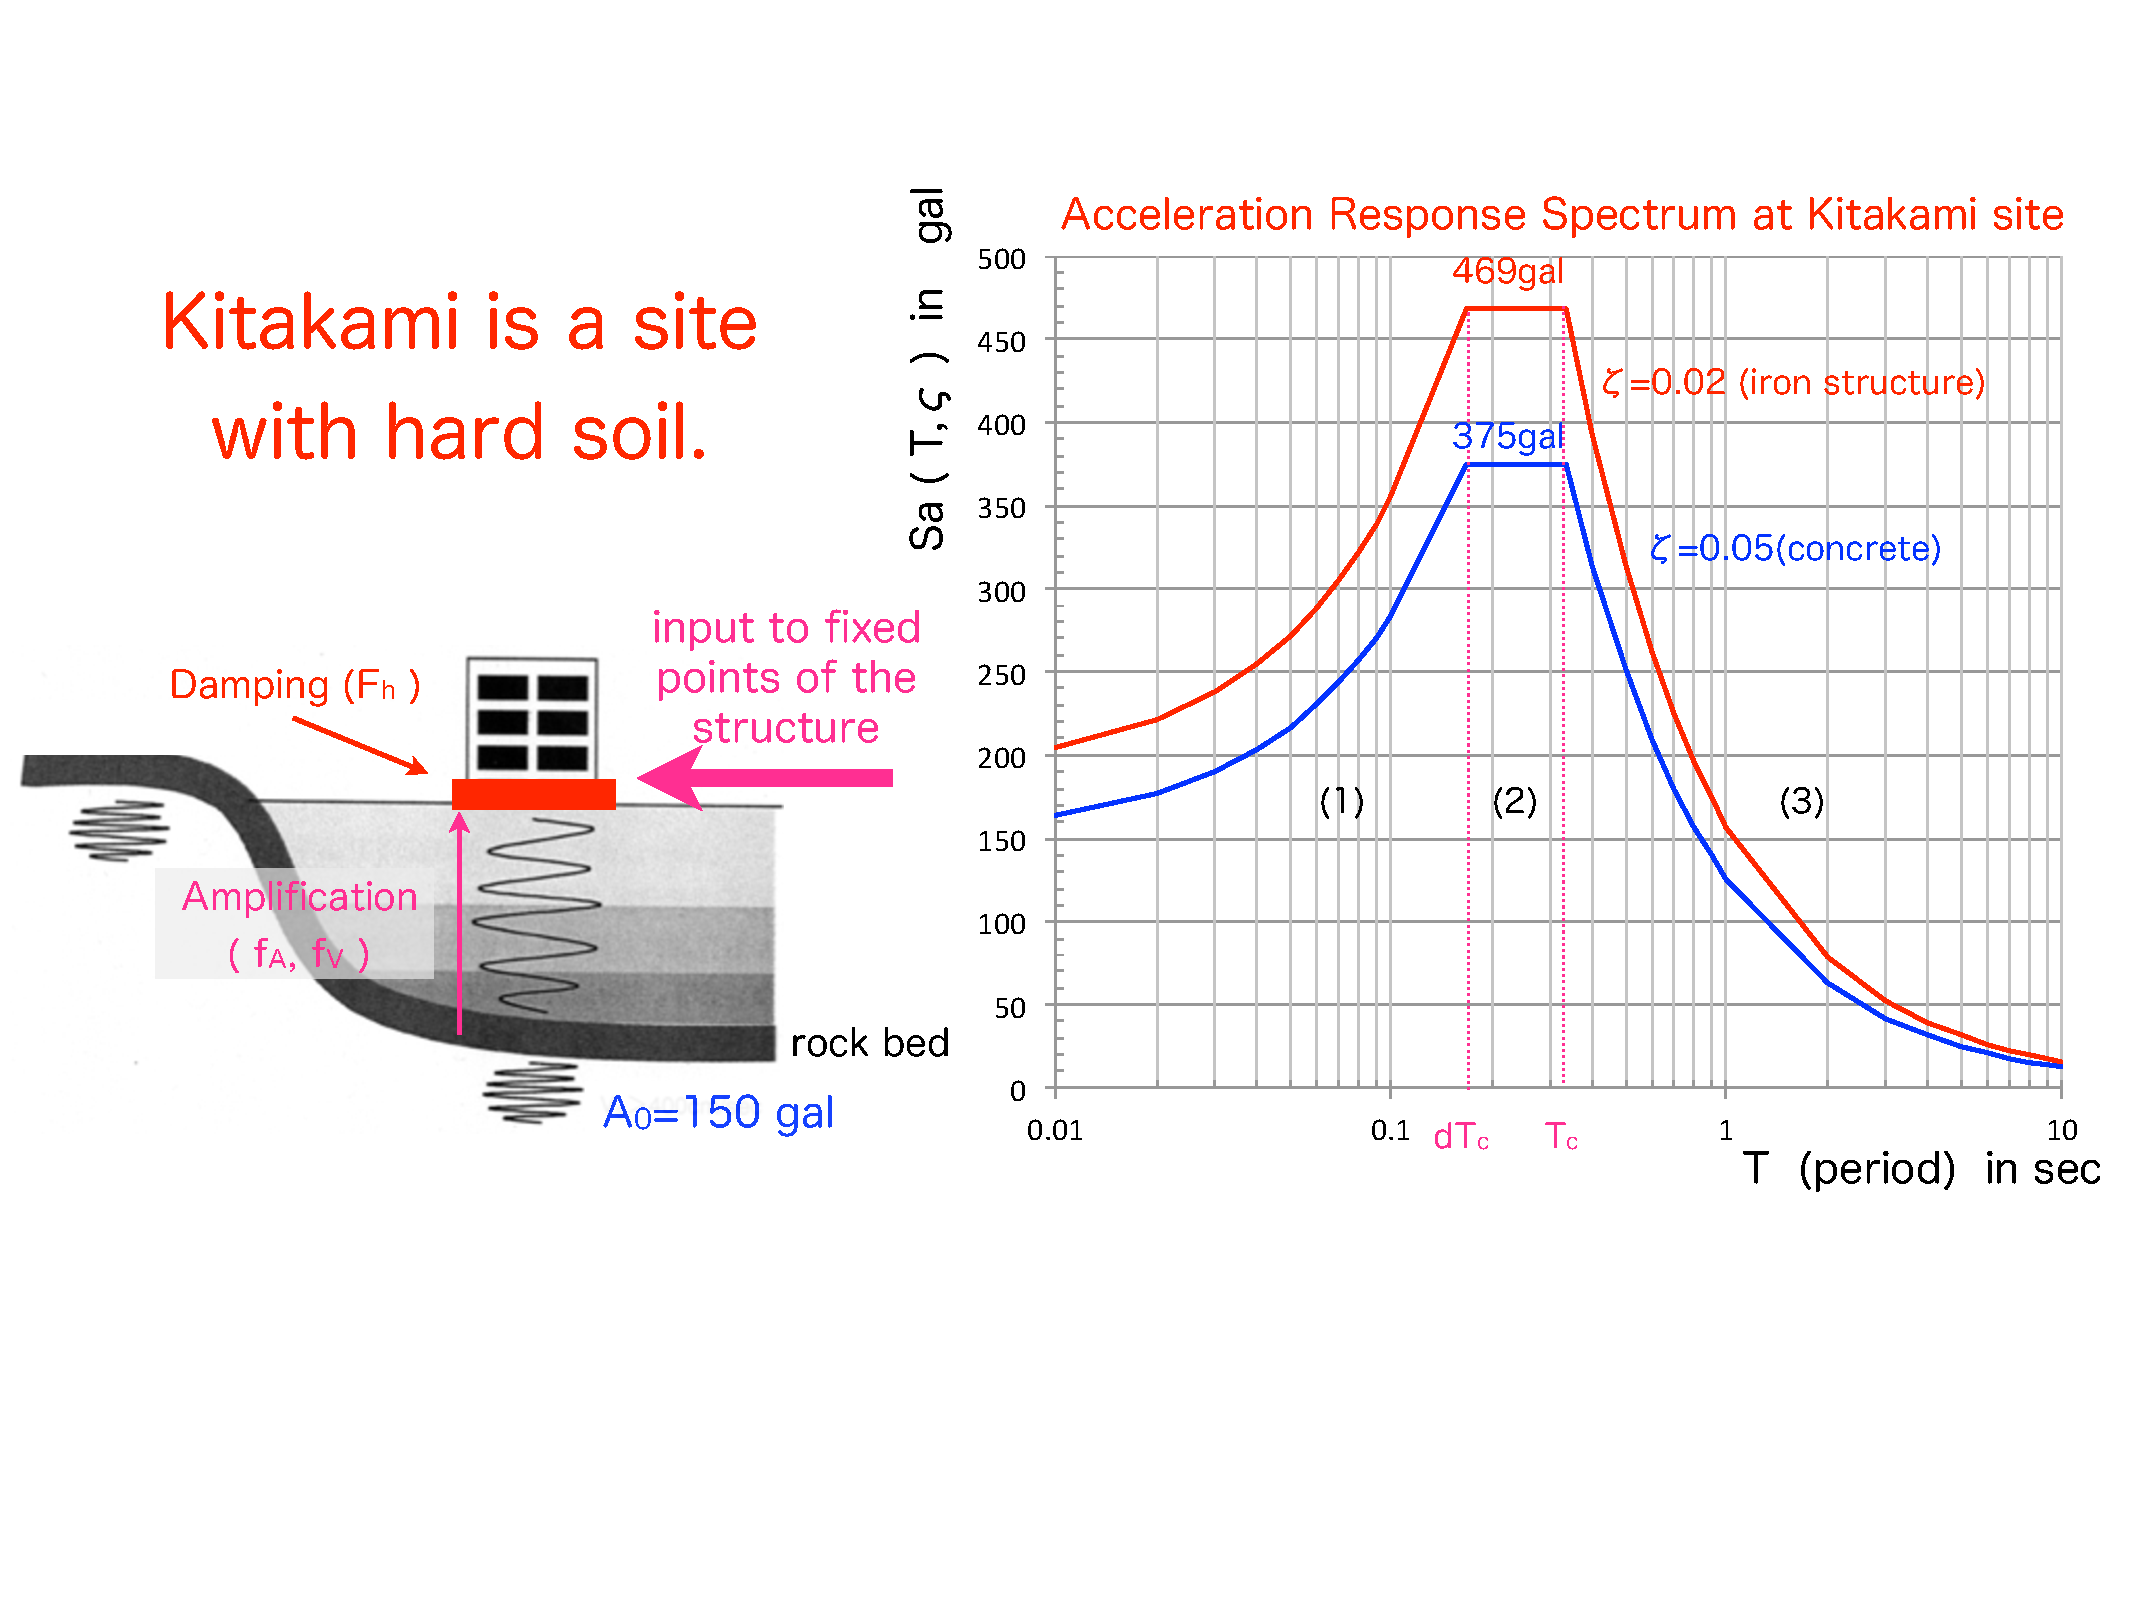
\includegraphics[width=0.8\hsize]{Integration/fig/earthquake_spectra.pdf}
\caption{\label{ild:fig:integration:earthquake_spectra}Standard response spectra for earthquakes in Kitakami (hard soil) for structures with different damping behaviour~\cite{ild:bib:earthquake}. A maximum acceleration of 150~gal (1 gal = 1 cm/s$^2$) for an earthquake with a recurrence frequency of 100~years has been assumed.}
\end{figure}

\subsection{Seismic Isolation}

Seismic isolation could be an attractive solution to mitigate the risk of earthquake induced accidents. Base isolation systems are in use in many cases in seismic active countries like Japan, under buildings, bridges and other critical infrastructure. A recent study~\cite{ild:bib:Seismic_Damping} has explored the possibility to install seismic damping systems underneath the ILD detector, e.g. under the detector platform. Standard isolation systems consist of rubber bearings in combination with oil dampers. Figure~\ref{ild:fig:integration:damping_earthquake} shows that accelerations acting on the ILD detector could be damped by a factor of $\approx$35 in case of a catastrophic earthquake. At the same time, such a system unfortunately increases the displacements of the detector in case of seismic mircrotremors that occur frequently in Japan, also at the Kitakami site~(c.f.~Figure~\ref{ild:fig:integration:earthquake_map}). An extended system that adds a rigid sliding bearing could mitigate the problem. Here, friction keeps the detector coupled to the ground at lower acceleration forces. Figure~\ref{ild:fig:integration:damping_microtremor} shows that no amplification of microtremors happens in that case. At the same time, the damping behaviour in case of major earthquakes is still in the order of a factor of $\approx$22 better than without base isolation~(Figure~\ref{ild:fig:integration:damping_earthquake}). 

\begin{figure}[h!]
\begin{center}
\begin{subfigure}{0.9\hsize} 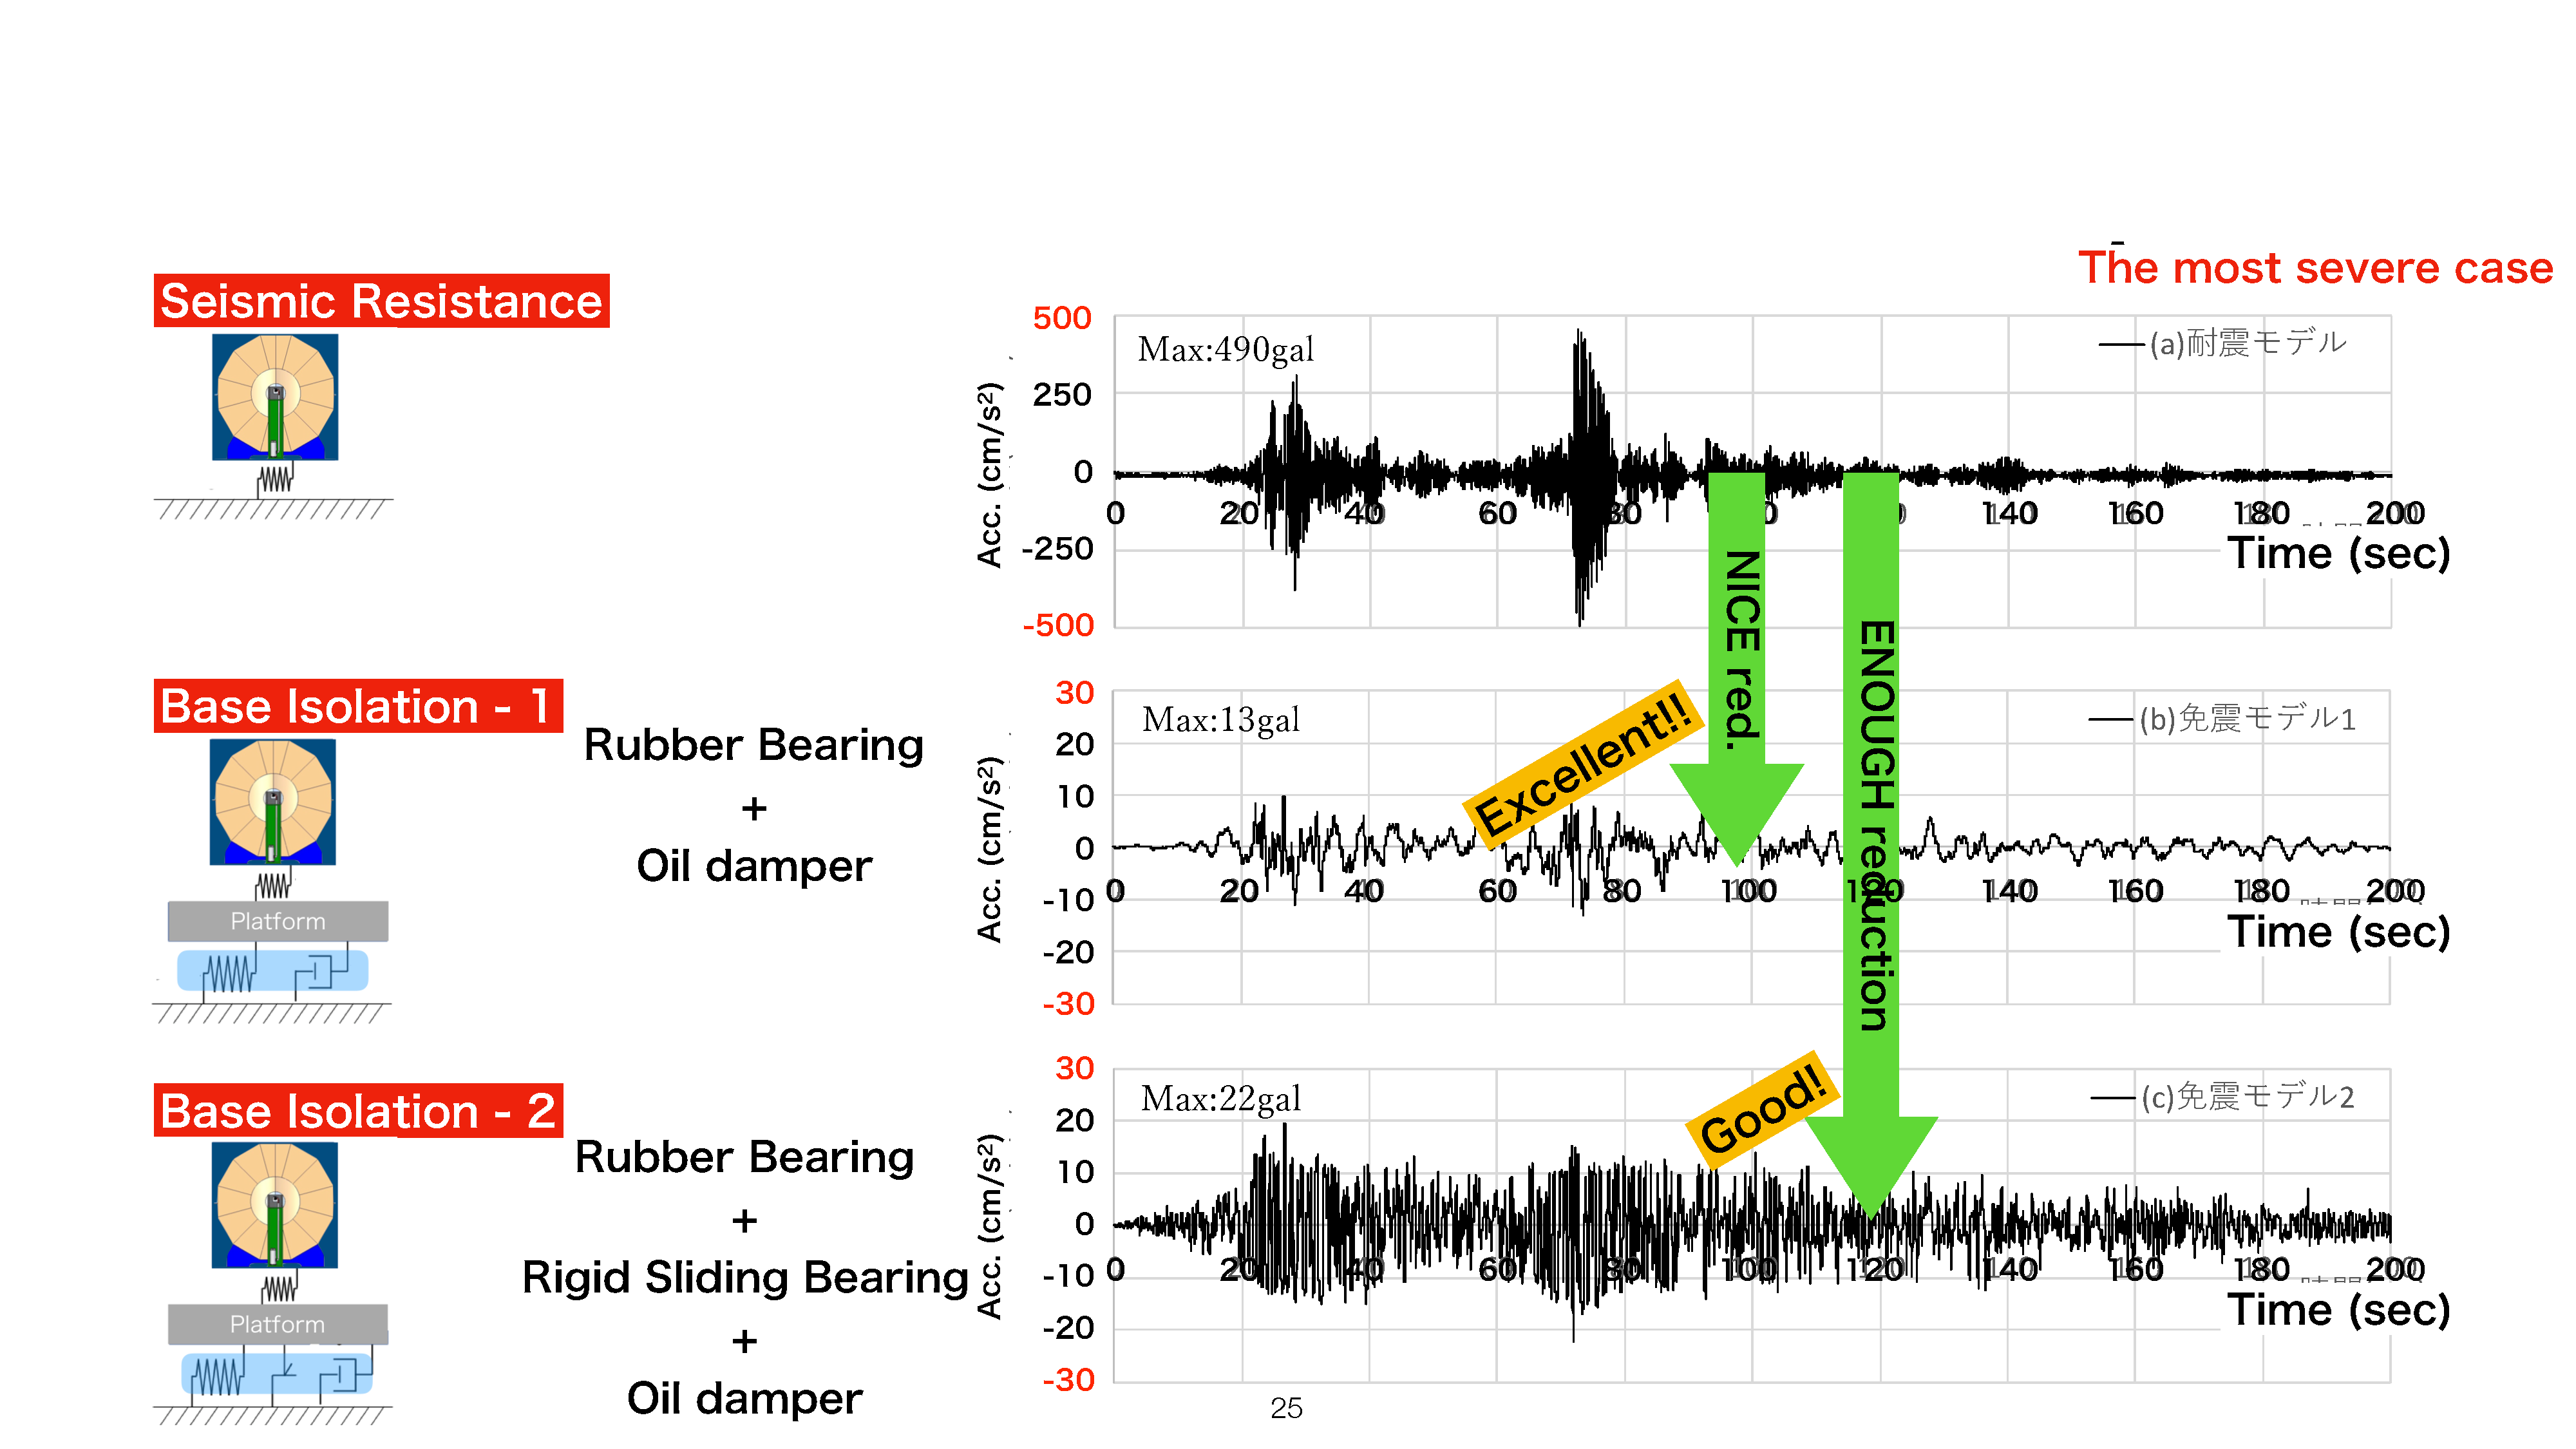
\includegraphics[width=\textwidth]{Integration/fig/Damping_Earthquake.pdf}
 \caption{ \label{ild:fig:integration:damping_earthquake}}
 \end{subfigure}
\hspace{0.03\textwidth}
\begin{subfigure}{0.9\hsize} 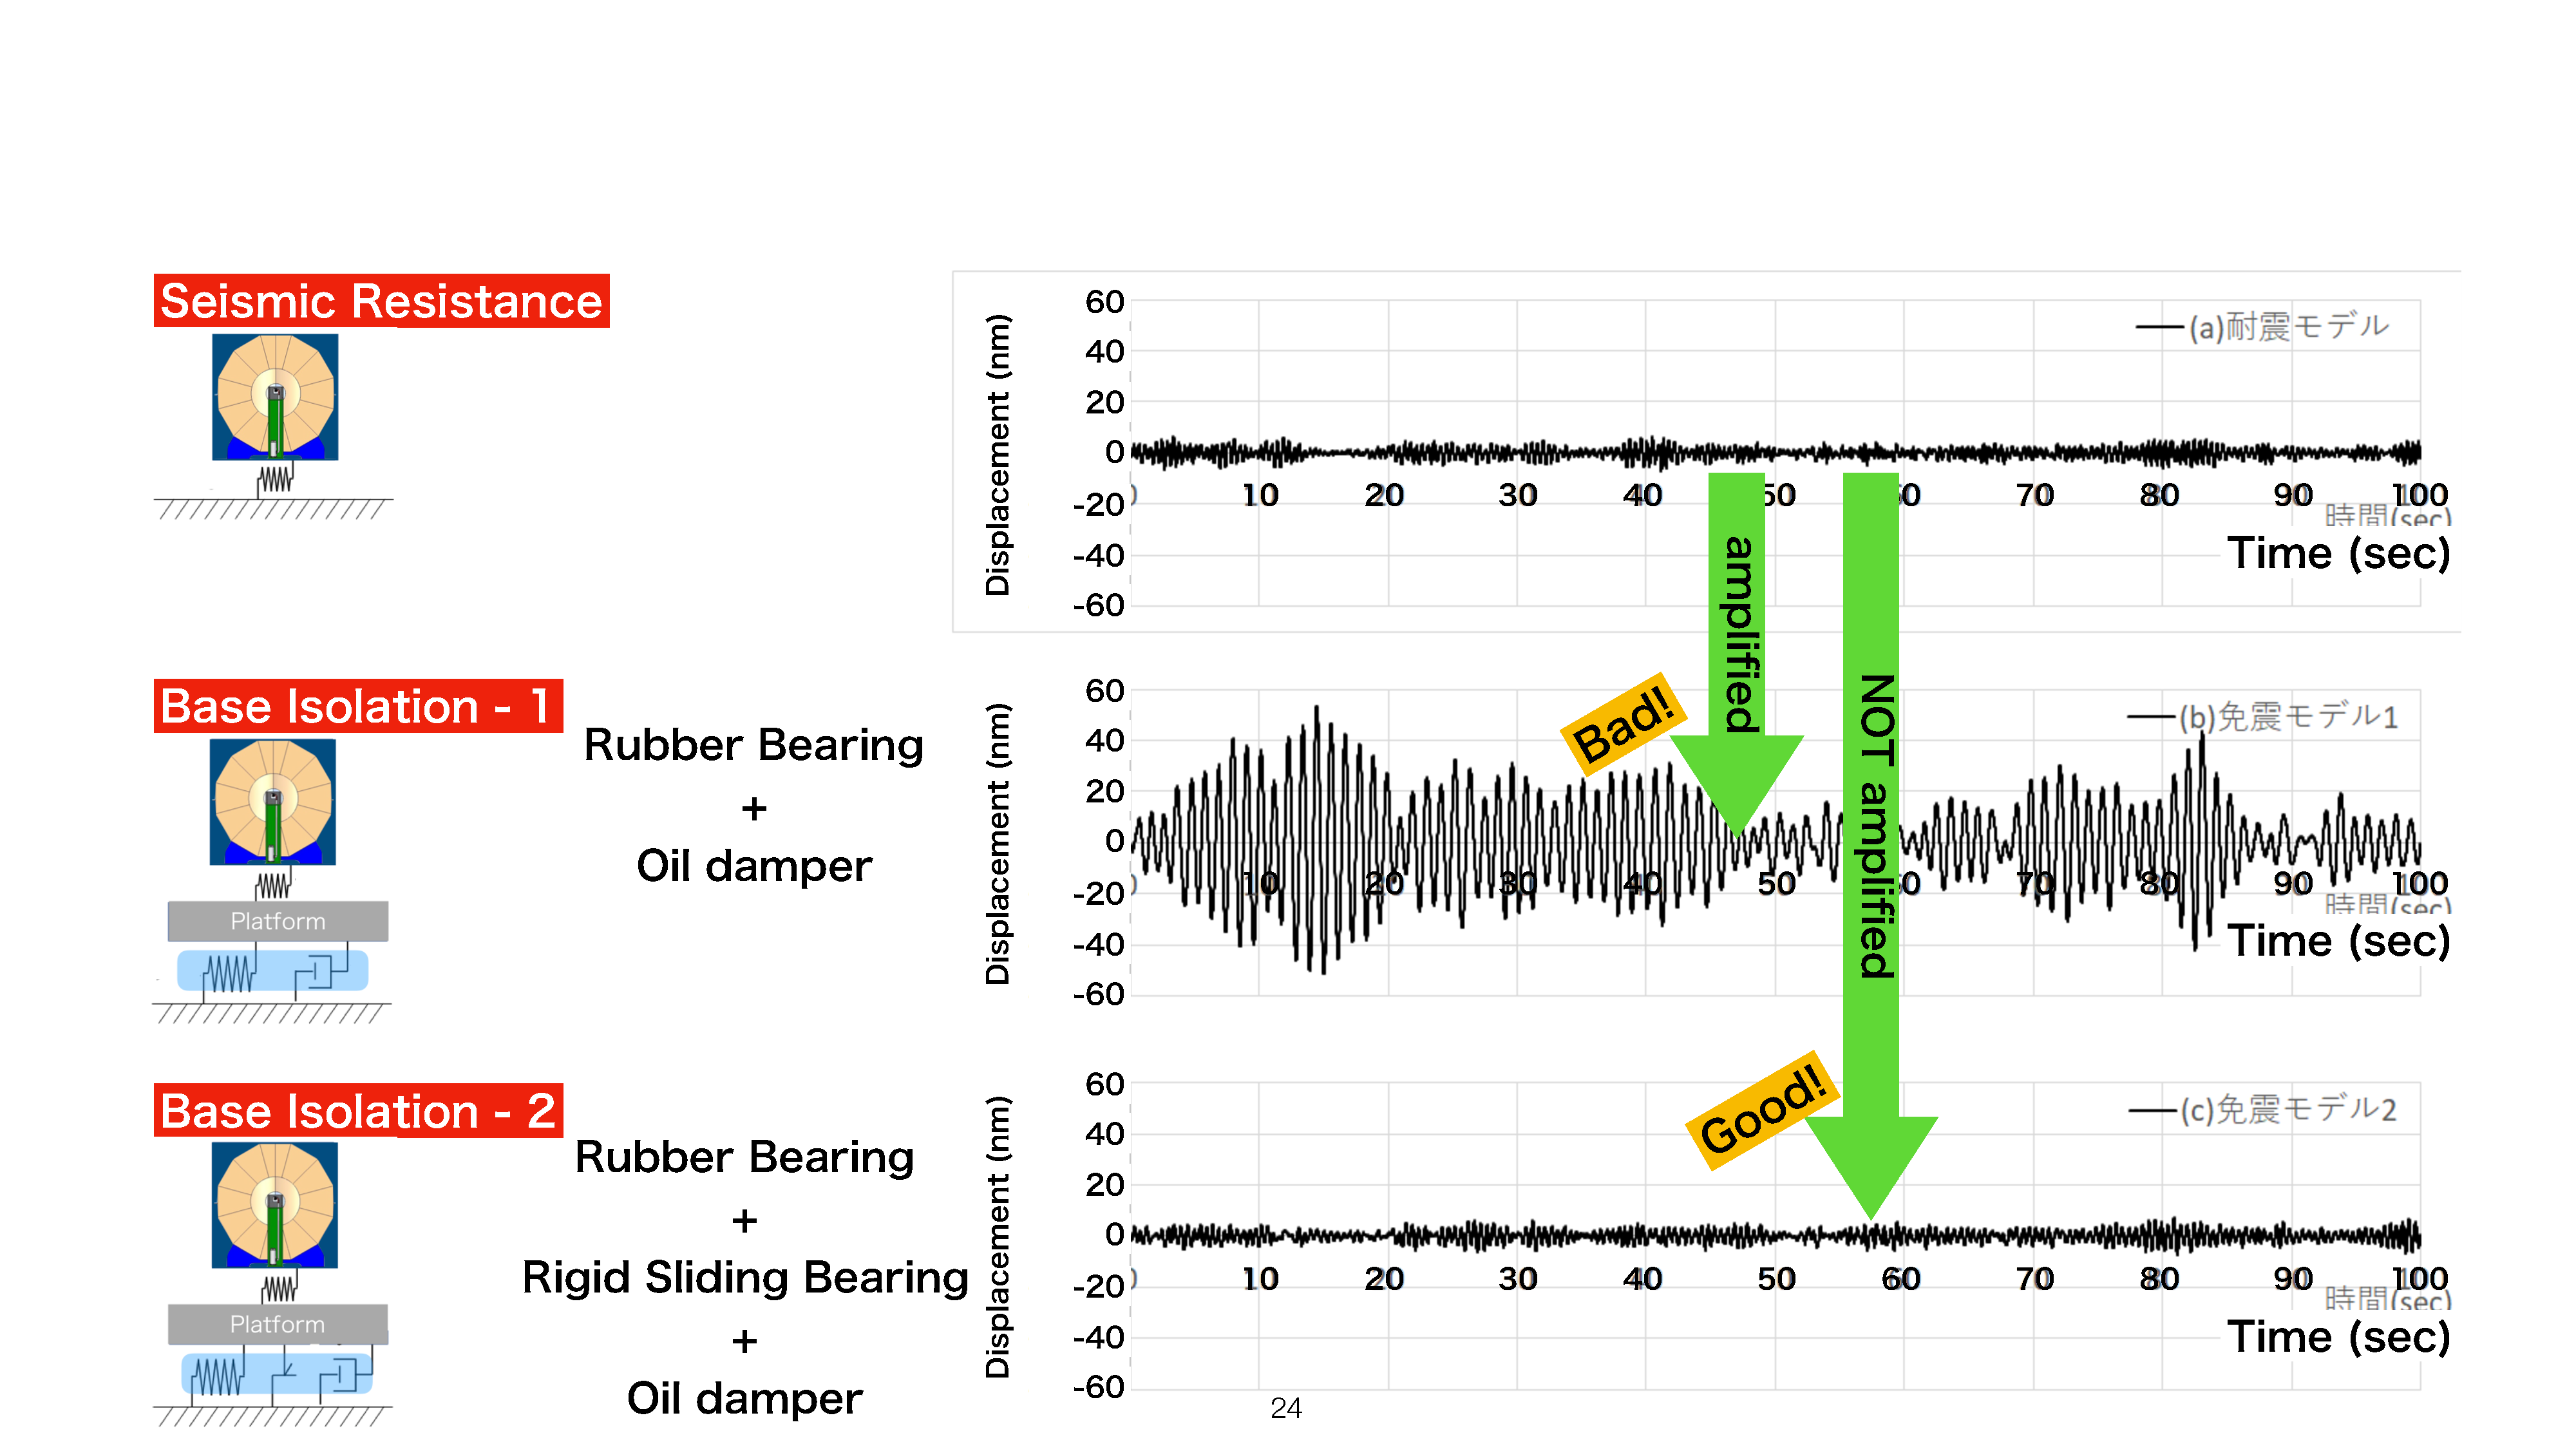
\includegraphics[width=\textwidth]{Integration/fig/Damping_Microtremor.pdf}
 \caption{  \label{ild:fig:integration:damping_microtremor}}
 \end{subfigure}
\end{center}
\caption{
(a) Simulated accelerations on the ILD detector in case of a catastrophic earthquake without base isolation (top) with an rubber bearing/oil damper system (middle) and with an additional rigid sliding bearing (bottom). Acceleration spectra from the 2011 Tohoku earthquake have been used as a case study for a most severe case~\cite{ild:bib:Seismic_Damping}.
(b) Simulated displacements of the ILD detector in case of microtremors without base isolation (top) with an rubber bearing/oil damper system (middle) and with an additional rigid sliding bearing (bottom) \cite{ild:bib:Seismic_Damping}.
}
\end{figure}


%\begin{figure}[h!]
%\centering
%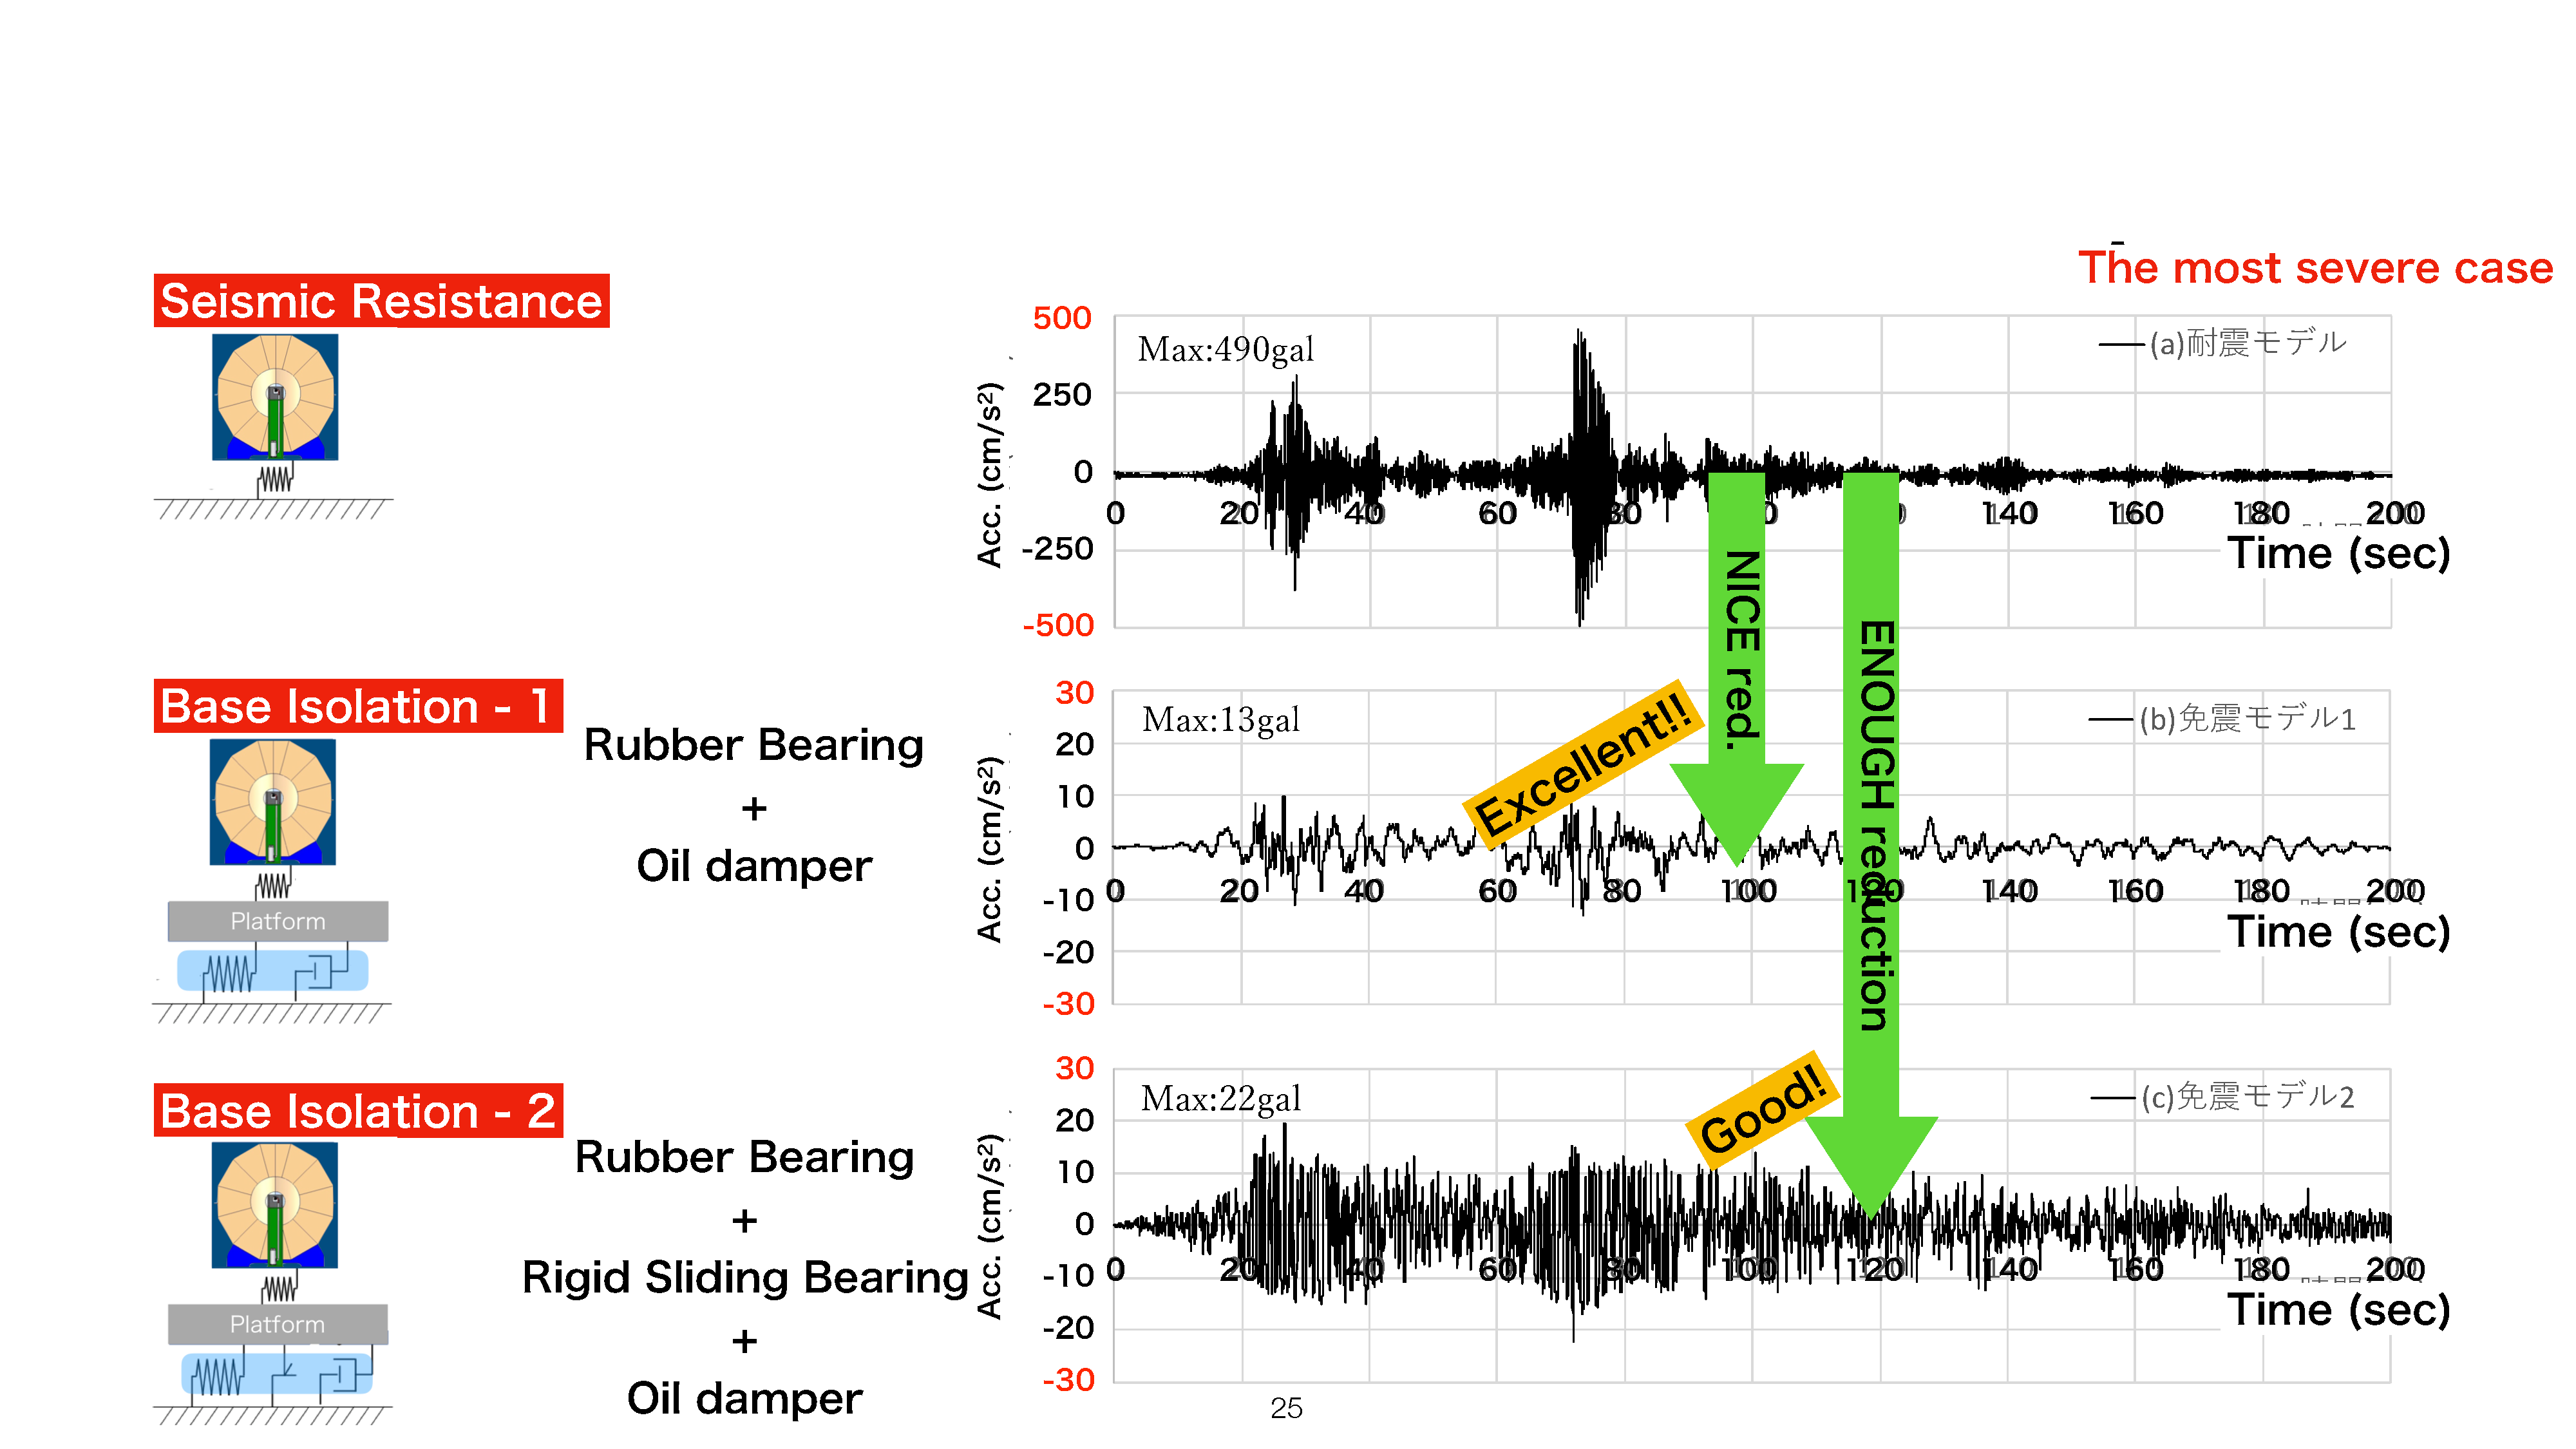
\includegraphics[width=0.8\hsize]{Integration/fig/Damping_Earthquake.pdf}
%\caption{\label{ild:fig:integration:damping_earthquake}Simulated accelerations on the ILD detector in case of a catastrophic earthquake without base isolation (top) with an rubber bearing/oil damper system (middle) and with an additional rigid sliding bearing (bottom). Acceleration spectra from the 2011 Tohoku earthquake have been used as a case study for a most severe case~\cite{ild:bib:Seismic_Damping}.}
%\end{figure}
%\begin{figure}[h!]
%\centering
%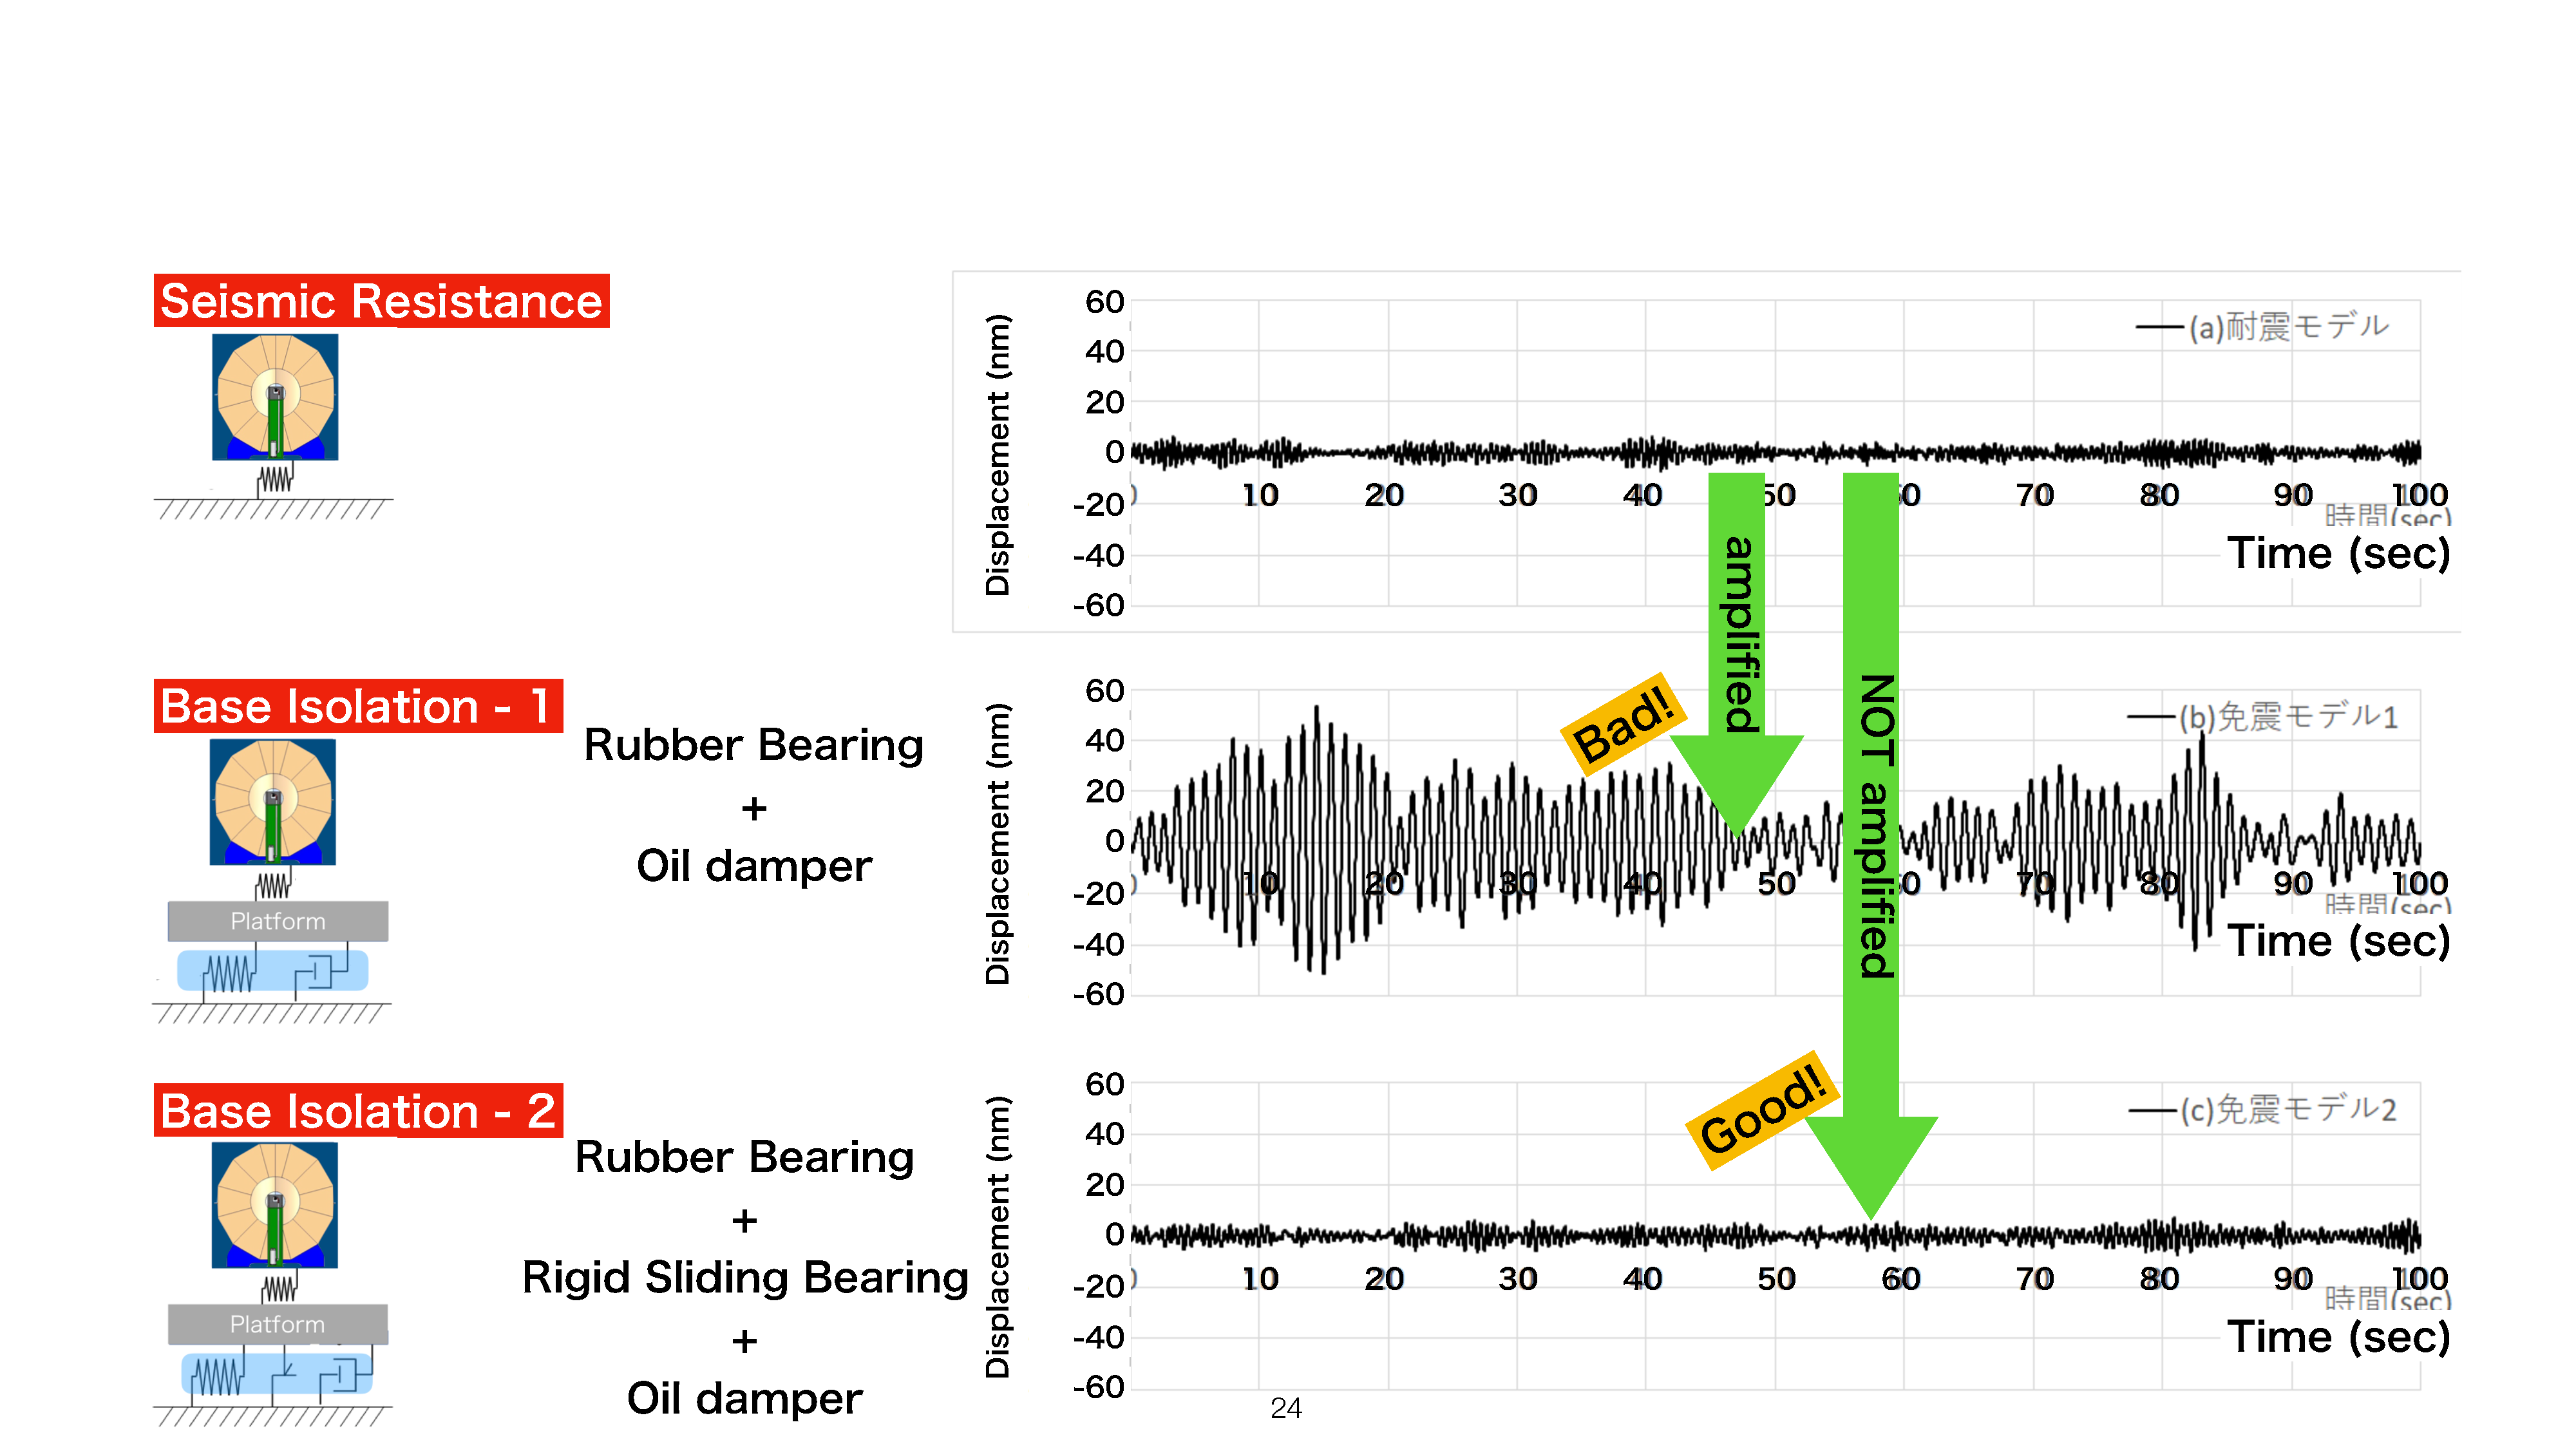
\includegraphics[width=0.8\hsize]{Integration/fig/Damping_Microtremor.pdf}
%\caption{\label{ild:fig:integration:damping_microtremor}Simulated displacements of the ILD detector in case of microtremors without base isolation (top) with an rubber bearing/oil damper system (middle) and with an additional rigid sliding bearing (bottom) \cite{ild:bib:Seismic_Damping}.}
%\end{figure}

A seismic base isolation system underneath the detector platform could therefore mitigate seismic risks for the ILD detector. However, earthquakes could also occur when the detector is still under construction or has been opened and moved partially away from the platform. Systematic risk evaluations and the development of mitigation strategies for the full lifetime of ILD still need to be done.
